% This example is meant to be compiled with lualatex or xelatex
% The theme itself also supports pdflatex
\PassOptionsToPackage{unicode}{hyperref}
\documentclass[aspectratio=1610, 9pt]{beamer}

% Load packages you need here
\usepackage{polyglossia}
\setmainlanguage{german}

\usepackage{csquotes}
    

\usepackage{amsmath}
\usepackage{amssymb}
\usepackage{mathtools}

\usepackage{hyperref}
\usepackage{bookmark}

% mine
\usepackage{algpseudocode}

% load the theme after all packages

\usetheme[
  showtotalframes, % show total number of frames in the footline
]{tudo}

% Put settings here, like
\unimathsetup{
  math-style=ISO,
  bold-style=ISO,
  nabla=upright,
  partial=upright,
  mathrm=sym,
}

\title{Bootstrapping Ansätze zur Bestimmung von Konfidenzbändern für Verteilungsfunktionen}
\author[D.~Richter]{Dennis Richter}
\institute[LS 4]{Lehrstuhl IV \\ Informatik}
\titlegraphic{
\includegraphics[width=0.55\textwidth]{images/tudo-title-2.jpg}}


\begin{document}

\maketitle

\begin{frame}
  \frametitle{Motivation und Problemstellung}
  \begin{center}
    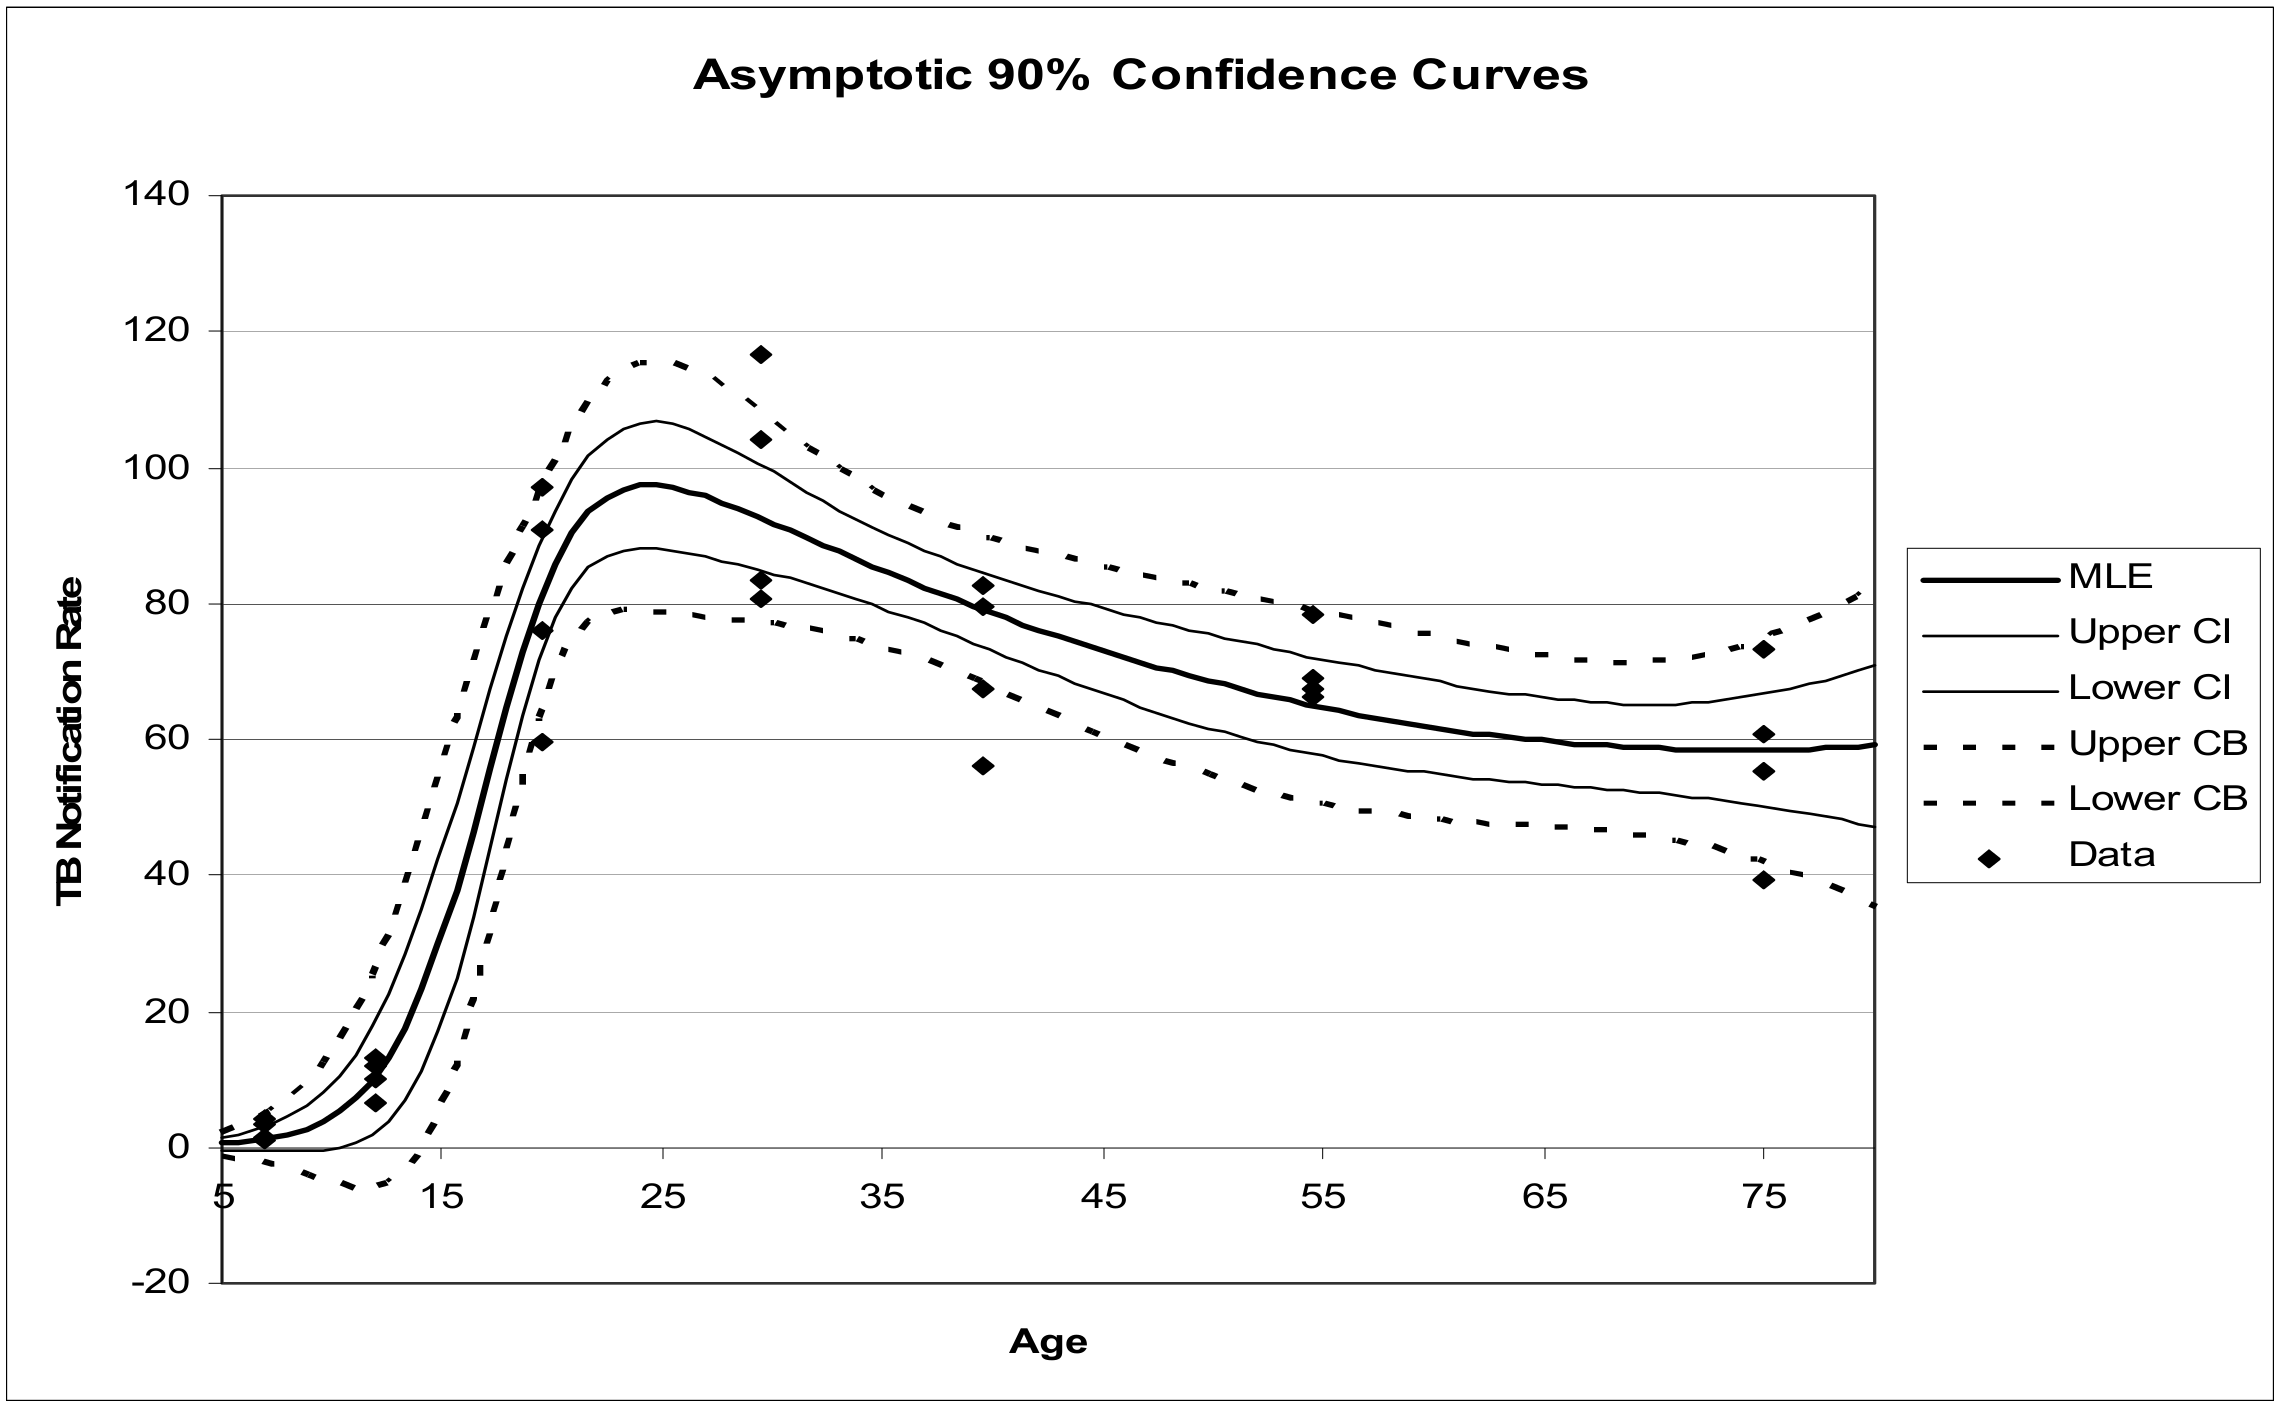
\includegraphics[width=0.7\textwidth]{images/4.png}
  \end{center}
\end{frame}

\begin{frame}
  \frametitle{Motivation und Problemstellung}
  \begin{itemize}
    \item Konfidenzintervalle sind visuelle Hilfsmittel zur Interpretation der Genauigkeit einzelner Schätzwerte
    \item Konfidenzbänder werden für simultane Schätzungen benötigt
    \item Es gibt verschiedene Ansätze zur Bestimmung von Konfidenzbändern (analytische Verfahren, aber auch Bootstrap-Verfahren)
    \item In der Literatur gibt es viele theoretische Diskussionen über die Verwendung von Bootstrap zur Bestimmung von Konfidenzbändern, aber wenige Implementierungen und empirische Ergebnisse
  \end{itemize}
\end{frame}

%\begin{frame}
%  \frametitle{PIBA - vier Stichpunkte (anstatt Gliederungsfolie)}
%\end{frame}

\begin{frame}
  \frametitle{Grundlagen}
  \begin{itemize}
    \item Regressionsfunktion $\eta(x, \theta)$: \\ 
    gesucht ist $\theta_0$ mit $y_j = \eta(x_j, \theta_0) + \epsilon_j$, $j = 1,2...,n$ und $\epsilon \sim N(0, \sigma^2)$ \\
    \item Schätzer $\hat{y}(x) = \eta(x, \hat\theta)$ für den "wahren Wert" $E(y|x) = \eta(x, \theta_0)$ \\
    \item Konfidenzbereich für den Schätzer: \\
    $P\left( \theta_L \le \theta_0 \le \theta_U \right) \geq 1-\alpha$
    \\
    z.B. $\theta_L, \theta_U = \hat\theta \mp z_{\alpha/2}\sqrt{\mathbf{V}(\hat\theta)}$
    \\
    \item Konfidenzintervall für einen Punkt der Regressionsfunktion: \\
    $\forall x: P\left(y_L(x) \le \eta(x, \theta_0) \le y_U(x)\right) \geq 1-\alpha$
    \\
    z.B. $y_L(x), y_U(x) = \eta(x, \hat\theta) \mp 
    z_{\alpha/2}
    \sqrt{
      \left(
        \frac{\partial\eta(x, \theta)}{\partial\theta}
      \right)_{\hat\theta}^T
      \mathbf{V}(\hat\theta)
      \left(
        \frac{\partial\eta(x, \theta)}{\partial\theta}
      \right)_{\hat\theta}
    }$
    \item Konfidenzband für die Regressionsfunktion: \\
    $P\left(\forall x: y_L(x) \le \eta(x, \theta_0) \le y_U(x) \right ) \geq 1-\alpha$
    \\
    z.B. $y_L(x), y_U(x) = \eta(x, \hat\theta) \mp 
    \sqrt{
      \chi_p^2(a)
      \left(
        \frac{\partial\eta(x, \theta)}{\partial\theta}
      \right)_{\hat\theta}^T
      \mathbf{V}(\hat\theta)
      \left(
        \frac{\partial\eta(x, \theta)}{\partial\theta}
      \right)_{\hat\theta}
    }$
  \end{itemize}
\end{frame}

\begin{frame}
  \frametitle{Grundlagen}
  \hspace{20px} \vline \hspace{5px}   
  \begin{minipage}[t]{0.3\linewidth}
    Basic-Sampling-Methode: \\
    \begin{algorithmic}
			\For {$j=0$ to $B$}
				\For {$i=0$ to $n$} 
				  \State Draw sample $y_{ij}$ from $F(.)$
				\EndFor
				\State Calculate statistic $s_j = s(y_j)$
			\EndFor
			\State Form the EDF $G_n(.|s)$
	  \end{algorithmic}
  \end{minipage}
  \hspace{10px} \vline \hspace{5px}
  \begin{minipage}[t]{0.48\linewidth}    
    Bootstrap-Methode: \\
    \begin{algorithmic}
      \Require Random sample $y = (y_1, y_2, ...y_n)$ from $F(.)$
      \State Form the EDF $F_n(.|y)$
			\For {$j=0$ to $B$}
				\For {$i=0$ to $n$} 
				  \State Draw sample $y^*_{ij}$ from $F_n(.|y)$
				\EndFor
				\State Calculate statistic $s^*_j = s(y^*_j)$
			\EndFor
			\State Form the EDF $G_n(.|s*)$
	  \end{algorithmic}
  \end{minipage}
\end{frame}

\begin{frame}
  \frametitle{Verwandte Arbeiten} 
  \begin{itemize}
    \item Cheng, Russell. (2005). Bootstrapping simultaneous confidence bands. 8 pp.-. 10.1109/WSC.2005.1574257.
    \item Cheng, Russell. (2015). Bootstrap confidence bands and goodness-of-fit tests in simulation input/output modelling. 16-30. 10.1109/WSC.2015.7408150.
    \begin{center}
      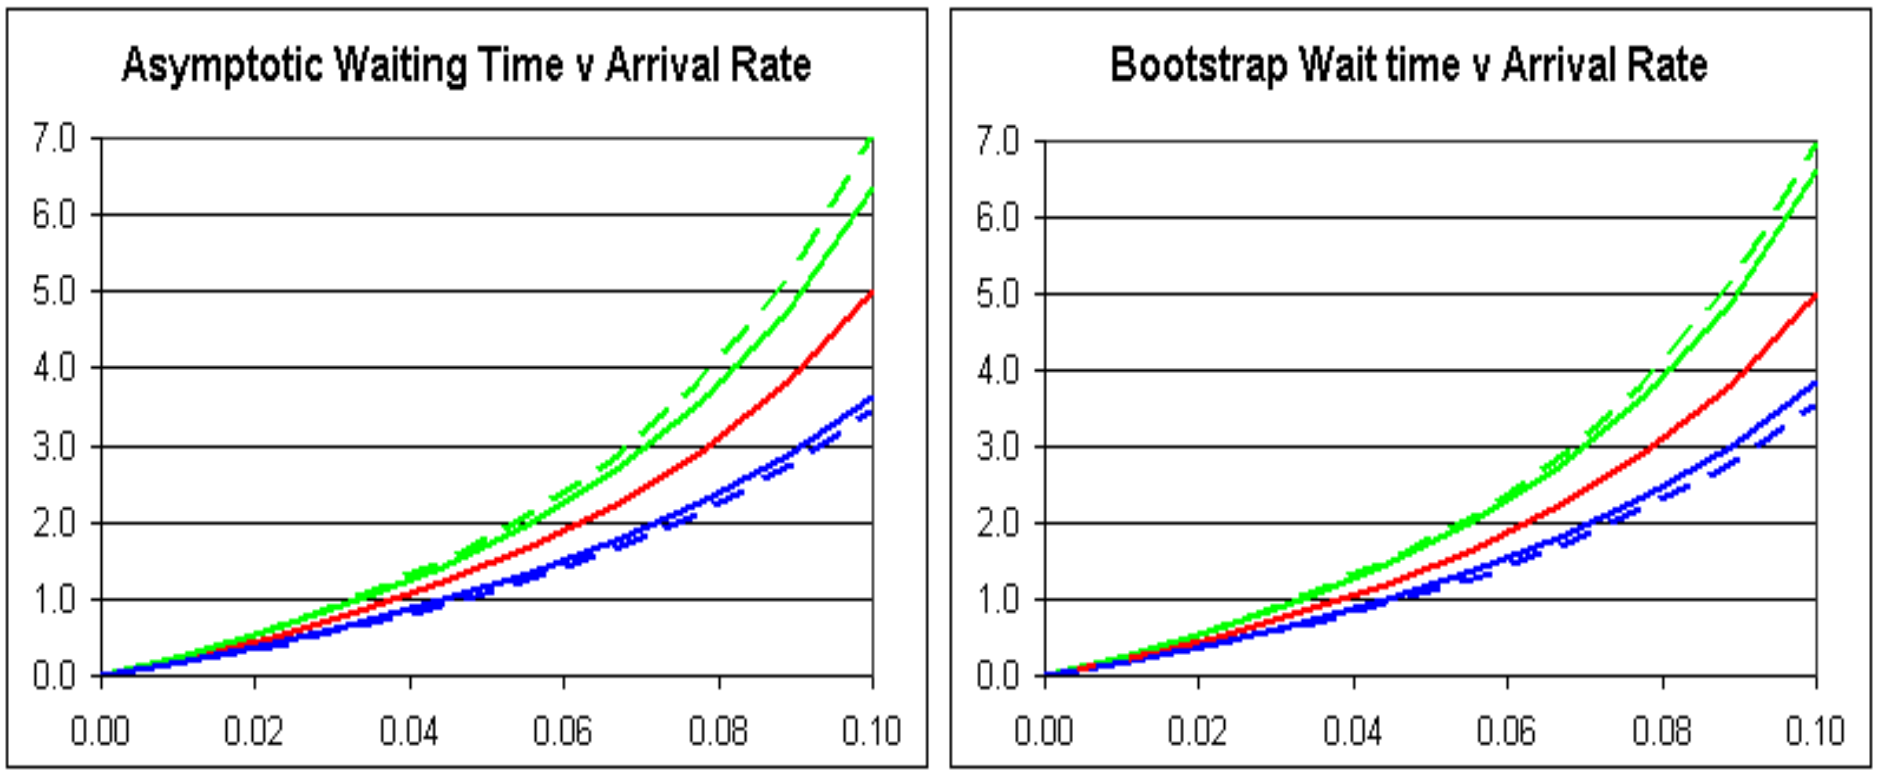
\includegraphics[width=0.5\textwidth]{images/3.png}
    \end{center}
  \end{itemize}
  Weitere:
  \begin{itemize}
    \item Govind, Nirmal \& Roeder, Theresa. (2006). Estimating Expected Completion Times with Probabilistic Job Routing. 1804-1810. 10.1109/WSC.2006.322958. 
    \item Wang, Xing \& Wang, Xin \& Sun, Zhaonan. (2009). Comparison on Confidence Bands of Decision Boundary between SVM and Logistic Regression. 272-277. 10.1109/NCM.2009.281.
  \end{itemize}
\end{frame}

\begin{frame}
  \frametitle{Lösungsansatze}
  2 Ansätze werden vorgestellt, bei denen Bootstrap zur Vereinfachung der analytischen Verfahren verwendet wird
  \begin{itemize}
    \item Parametric Bootstrap:
    \begin{itemize}
      \item setzt voraus, dass $\hat\theta$ als normalverteilt angenommen werden kann, d.h. $\hat\theta \sim N(\theta_0, \mathbf{V}(\theta_0))$
      \item verzichtet jedoch auf die lineare Approximation von $\eta(x,\theta)$ durch die Delta-Methode
    \end{itemize}
    \item Non-Parametric Bootstrap:
    \begin{itemize}
      \item keine Verteilungsannahme über $\hat\theta$
      \item und auch keine lineare Approximation von $\eta(x,\theta)$
      \item rechenintensiv wegen verschachteltem Doppel-Bootstrap 
    \end{itemize}
  \end{itemize}
  Es gibt jedoch auch andere analytische Verfahren zur Bestimmung von Konfindenzbändern, bei denen Bootstrap verwendet werden kann
\end{frame}

\begin{frame}
  \frametitle{Anwendnungs Beispiel}
  \begin{minipage}[t]{0.48\linewidth}
	  \begin{figure}
	    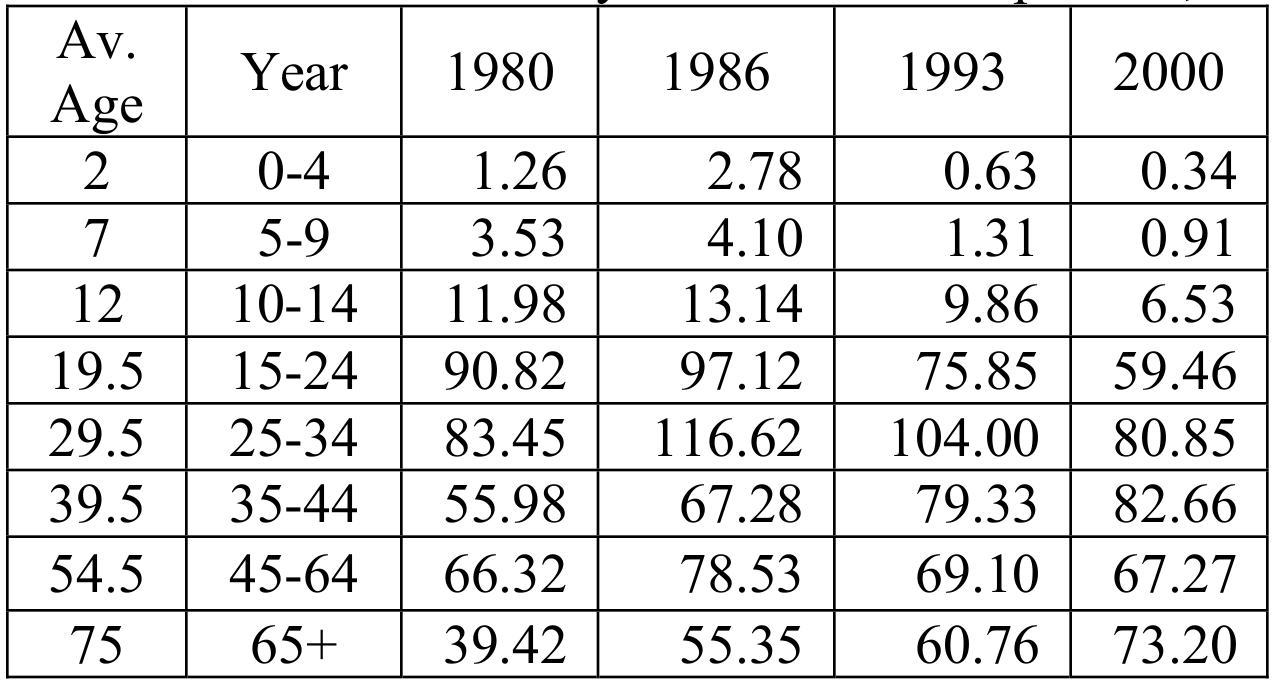
\includegraphics[width=0.8\textwidth]{images/5.png}
	    \caption{Morocco Pulmonary TB notifications per 100,000}
	  \end{figure}
  \end{minipage} 
  \begin{minipage}[t]{0.48\linewidth}
	  \begin{figure}
	    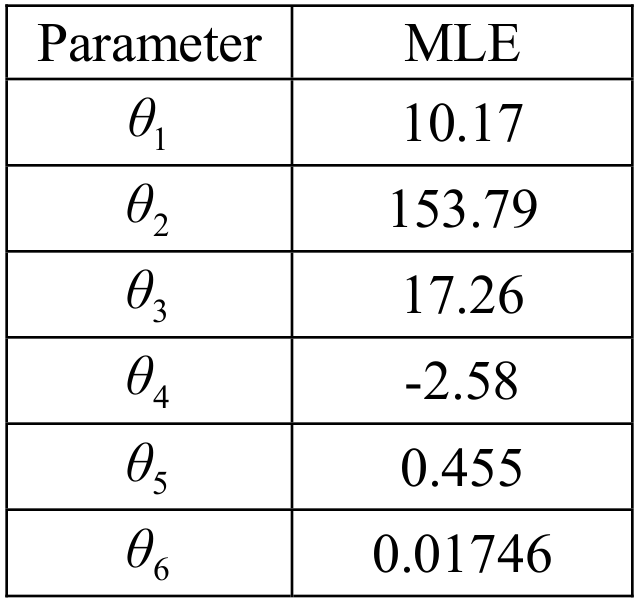
\includegraphics[width=0.4\textwidth]{images/6.png}
	    \caption{MLE’s for the Morocco TB Model}
	  \end{figure}
	\end{minipage}
	\begin{figure}
	  Als Modell wurde gewählt: 
		\begin{align*}
		    y_j = (\theta_2 + \theta_4 x_j + \theta_6 x^2_j)
			  \frac{
			    exp(\theta_5(x_j - \theta_3))}{
			    1 + exp(\theta_5(x_j - \theta_3))
			  } + \epsilon_j
		\end{align*}
		wobei $\epsilon_j \sim N(0, \theta_1^2)$
	\end{figure}
\end{frame}

\begin{frame}
  \frametitle{Anwendnungs Beispiel}
  \begin{center}
    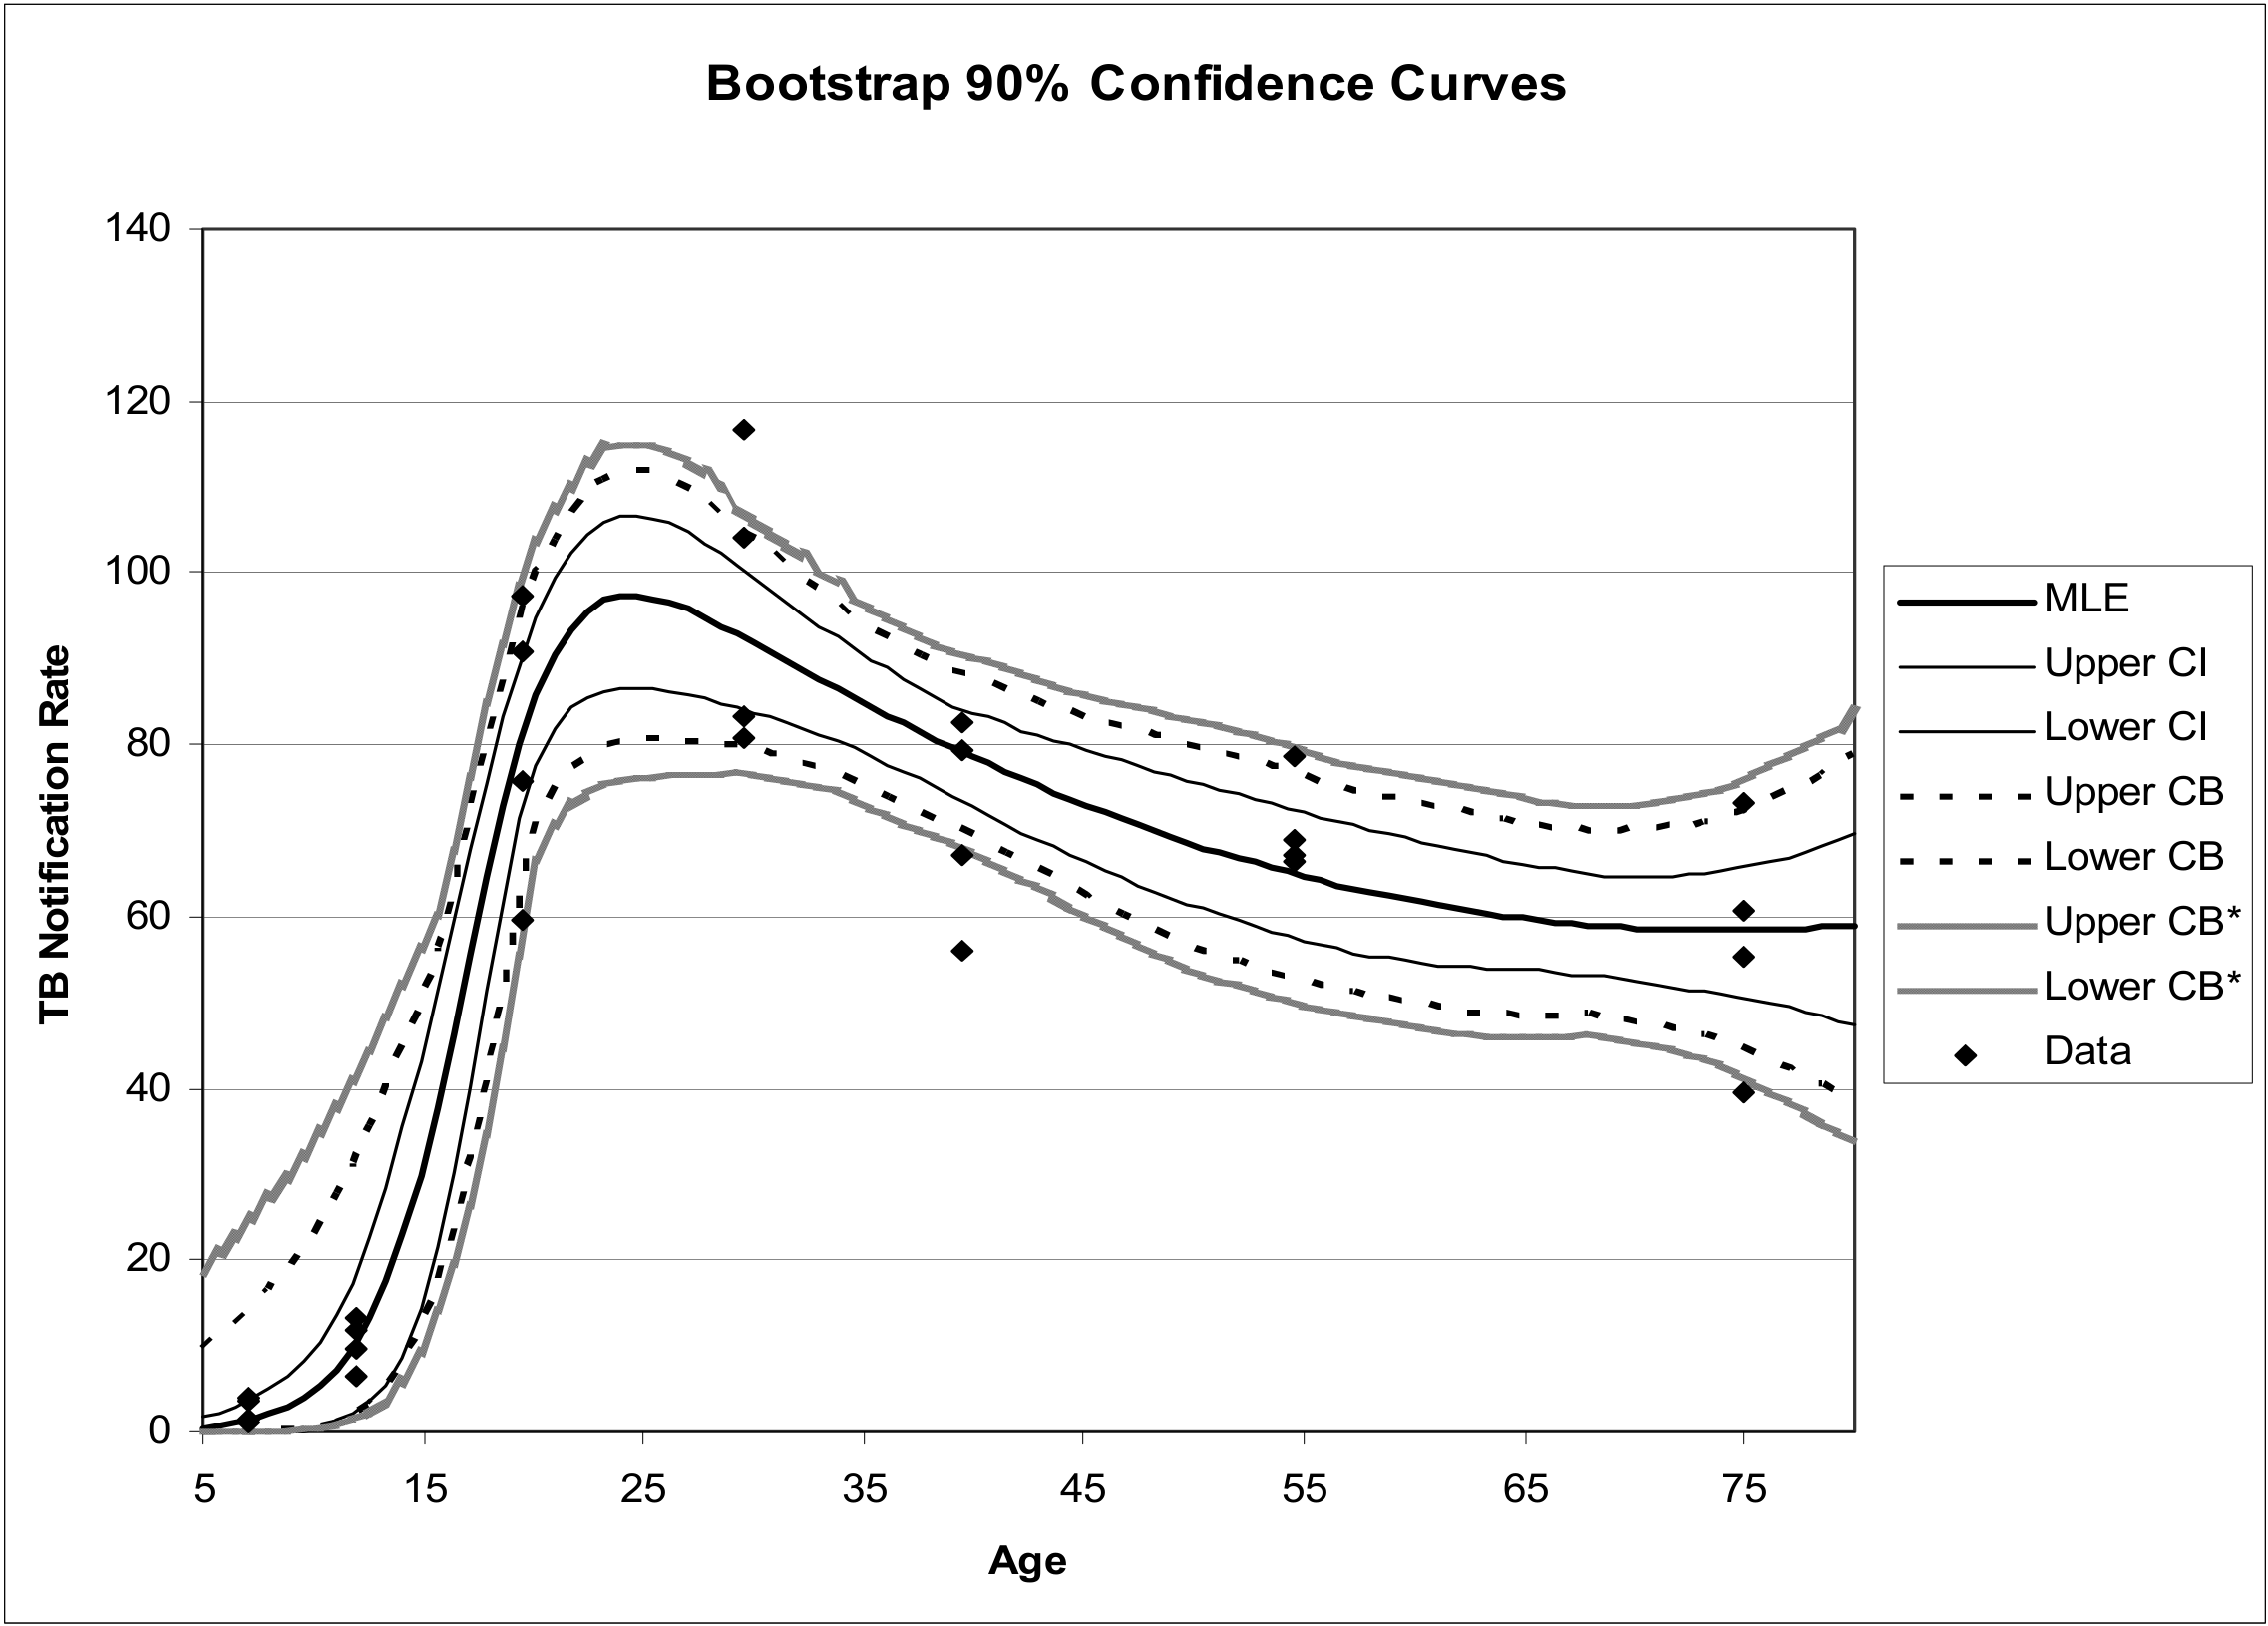
\includegraphics[width=0.6\textwidth]{images/1.png}
  \end{center}
\end{frame}

\begin{frame}
  \frametitle{Umsetzung}
  \begin{itemize}
    \item 2 Wochen: Vertiefende Recherche der Bootstrap-Ansätzen 
    \item 1 Woche: Recherche zu Parameterstudien, Auswertung und Darstellung in Kontext von OMNeT++
    \item 1 Woche: Erstellung von mindestens 2 einfachen Beispielen in Form einer OMNeT++ Simulation
    \item 2 Wochen: Implementierung der Verfahren in C++ (mindestens die von Cheng (2005) vorgestellten Ansätze)
    \item 2 Wochen: Anwendung der Verfahren und empirische Bewertung
  \end{itemize}
  Zudem:
  \begin{itemize}
    \item Die implementierung soll wiederverwendbar sein (über Git) und nach Möglichkeit in die IDE integriert
    \item Zwischen den Arbeitspaketen sind jeweils Schreibphasen geplant
  \end{itemize}
\end{frame}

\begin{frame}
  \frametitle{Geplante Evaluation}
  Die Verfahren werden anhand der zuvor erstellten Beispiele getestet:
  \begin{itemize}
    \item Datenerhebung durch die Simulation 
    \item Bestimmung eines statistischen Modells und der Regressionsgerade (Modellanpassung)
    \item Auswertung mit analytischen Verfahren (durch C++-Libraries oder in R)
    \item Auswertung mit den implementierten Bootstrap-Verfahren
    \item Vergleich der Konfidenzbänder
  \end{itemize}
  Es wird erwartet, dass die Bootstrap-Ansätze ähnliche Konfidenzbänder liefern wie die analytischen Methoden und sich diesen annähern
\end{frame}

\begin{frame}
  \frametitle{Zeitplan}
  \begin{center}
    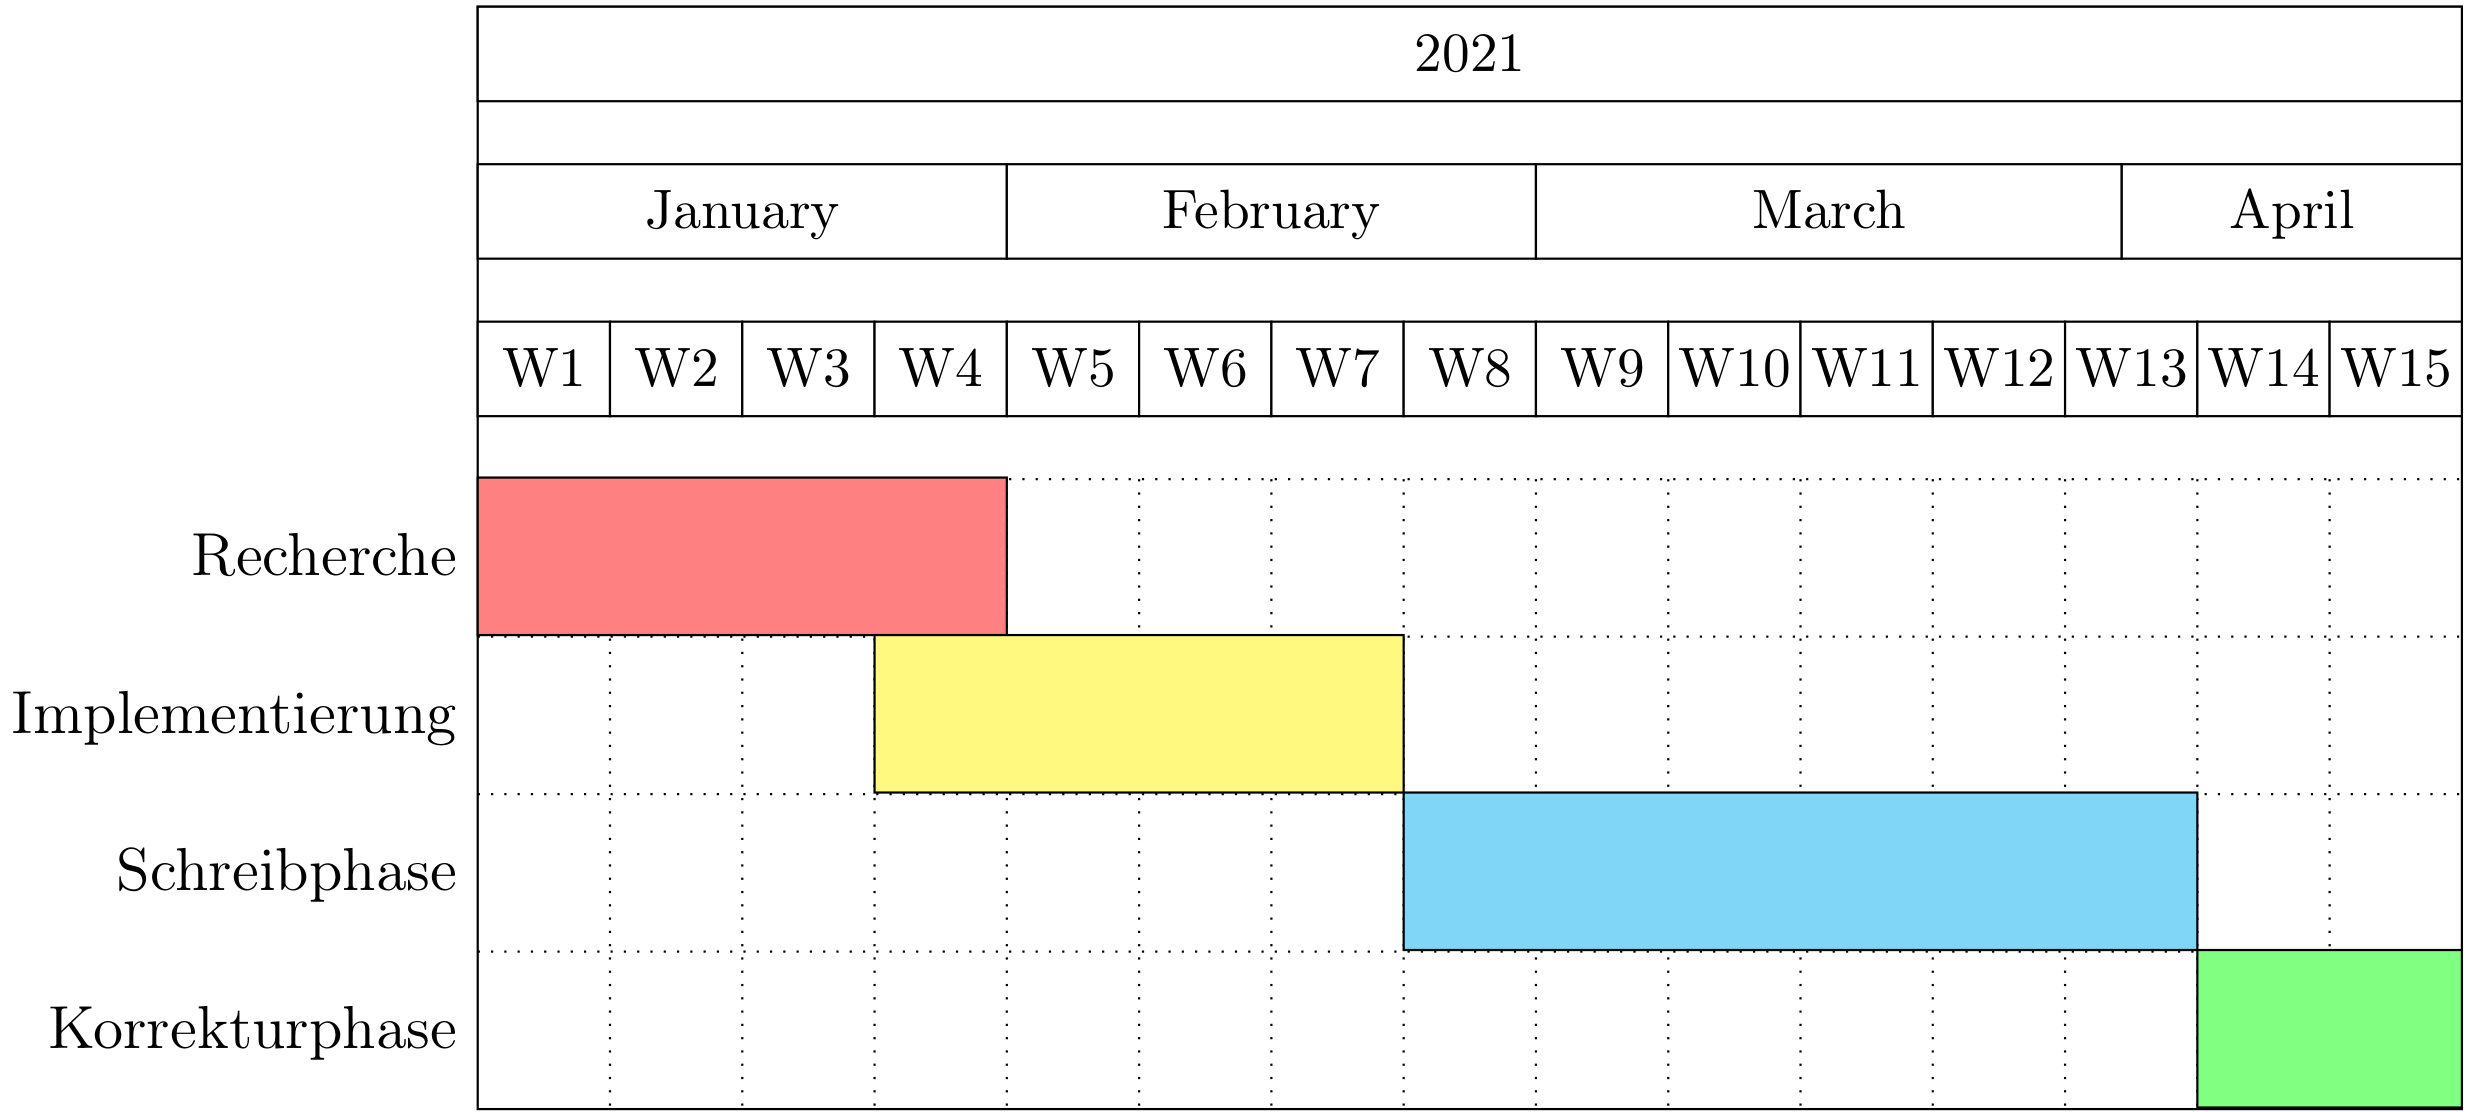
\includegraphics[width=0.8\textwidth]{images/2.png}
  \end{center}
\end{frame}

%	\begin{frame}
%	  \frametitle{PIBA - vier Stichpunkte (anstatt Gliederungsfolie)}
%	  \begin{itemize}
%	    \item Was ist das Problem? -> Implementierung von Bootstrap-Ansätzen zur Bestimmung von Konfidenzbändern
%	    \item Idee? -> Implementierung einiger Ansätze im Kontext von OMNeT++, Integration in die IDE nach Möglichkeit und Bewertung anhand von Simulationen
%	    \item Vorteil? -> Boostrap ist ein simples und allgemeines Verfahren und einsetzbar in ungewissen situationen -> die arbeit gibt einen erfahrungswert
%	    \item Aktion? -> zuerst die genannten und weitere Ansätze genauer recherchieren und vorstellen, dann in C++ im Kontext von OMNeT++ implementieren und nach Möglichkeit in die IDE integrieren, dann testen der Methoden anhand von einfachen Beispielen in Form einer OMNeT++ Simulation (z.B. ...)
%	  \end{itemize}
%	\end{frame}
\end{document}